\documentclass[../Final.tex]{subfiles}
\begin{document}

%Nomenclature table
\begin{table*}[t]
    \begin{framed}
    {
        \fontfamily{stix}\selectfont % select font nomenclature
        \fontsize{10}{12}\selectfont % font 12 pt nomenclature

        \nomenclature{$\alpha$}{exponent for Eq. (\hyperref[eq7]{7}) with range 1.5–1.7}		
        \nomenclature{$\beta$}{exponent for Eq. (\hyperref[eq7]{7}) with range 0.3–0.5 with $\alpha + \beta =2$}  
        \nomenclature{$\beta$}{hardening parameter}
        \nomenclature{$\delta$}{lateral indentation (mm)}
        \nomenclature{$\mathcal{E}$}{strain rate $(s^{-1})$}
        \nomenclature{$\mathcal{E}_{c}$}{critical rupture strain of the material 
        which is determined from where $\mathcal{E}_{c}=0.10(\mathcal{E}_{f} / 0.32)$ 
        where $\mathcal{E}_{f}$ is the steel material ductility obtained in tensile test}
        \nomenclature{$\mathcal{E}_{P}^{e f f}$}{effective plastic strain}
        \nomenclature{$\sigma_{0}$}{flow stress of the material (MPa)}
        \nomenclature{$\sigma_{o}$}{initial yield stress (Pa)}
        \nomenclature{$\sigma_{y}$}{yield stress (Pa)}
        \nomenclature{$C$}{Cowper-Symonds strain rate parameters $(s^{-1})$}
        \nomenclature{$c$}{cross-sectional length of a unit or the tearing length (mm)}
        \nomenclature{$d$}{average width of the plates in the crushed crosssection (mm)}
        \nomenclature{$D_{1}$}{coefficient related to the actual crushing or tearing configuration}


        \nomenclature{$D_{2}$}{coefficient related to the impact position and the plate size}
        \nomenclature{$E$}{Young’s modulus (Pa)}
        \nomenclature{$E$}{absorbed energy (MJ)}
        \nomenclature{$E_{p}$}{plastic hardening modulus (Pa)}
        \nomenclature{$E_{t a n}$}{Tangent modulus (Pa)}
        \nomenclature{$F_{m}$}{mean resistance (N)}
        \nomenclature{$F_{p}$}{resistance force (N)}
        \nomenclature{$H$}{height of rupture aperture in side shell (m)}
        \nomenclature{$L$}{critical tearing length (mm)}
        \nomenclature{$L_{N}$}{damage length of striking ship (m)}
        \nomenclature{$L_{n}$}{damage length of struck ship (m)}
        \nomenclature{$P$}{Cowper-Symonds strain rate parameters}
        \nomenclature{$P_{N}$}{damage depth of striking ship (m)}
        \nomenclature{$P_{n}$}{damage depth of struck ship (m)}
        \nomenclature{$R_{T}$}{destroyed material volume for both struck and striking ship/resistance factor (m3)}
        \nomenclature{$t_N$}{damage thickness of striking ship (m)}
        \nomenclature{$t_n$}{damage thickness of struck ship (m)}
        \nomenclature{$t_s$}{side shell thickness (cm)}

        \renewcommand*{\nompreamble}{\begin{multicols}{2}}
            \printnomenclature
        \renewcommand*{\nompostamble}{\end{multicols}}
    }
    \end{framed}
\end{table*}

The impact phenomenon may occur in several forms, espe­cially in marine and ocean engineering. As briefly described in previous section, collision is example of impact phenomenon in the mentioned field. 
Remarkable damages and wide range of casualties make involved parties to take collision load into calculation for their design. 
This condition encourages researchers to expand their study in impact engineering to marine and ocean fields with ship is main object in their studies. 


Several researches have been addressed for different ship types, including bulk carrier \cite{ozguc2005comparative}, tanker \cite{haris2013analysis,bae2016numerical}, barge \cite{leheta2014finite}, and passenger vessel \cite{prabowo2016evaluating,prabowo2016energy,prabowo2017analysis,prabowo2017effects}. 


Researches in collision have dominated by tanker in order to reduce possibility of oil spill, for instance by Yip et al. \cite{yip2011effectiveness}, and developed by several methods. 
The analytical method was developed by Hong and Amdahl in 2008 to calcu­lated crushing resistance of web girders \cite{hong2008crushing}. Experiment was also conducted by Lehmann and Peschmann \cite{lehmann2002energy} 
when they conducted collision test using NEDLLOYD 34 as the striking ship and AMATHA as the struck ship with cooperation of Germanischer Lloyd in 2002. After that empirical formula was used by Ozguc et al. \cite{ozguc2005comparative} 


When they used modified Minorsky formula to estimate internal energy based on damage pattern. Improvement of energy formula was taken into consideration by Bae et al. \cite{bae2016study}
as they used proposed energy formula by Zhang (Eqs. (\hyperref[eq1]{1})–(\hyperref[eq3]{3})). This formula is more speci.c than Minorsky as given in Eqs. (\hyperref[eq4]{4}) and (\hyperref[eq5]{5}) \cite{minorsky1958analysis}, and Woisin in Eq. (\hyperref[eq6]{6}) \cite{woisin1979design} as energy can be calculated based on different damage pattern. 


The damage modes of some basic structural element had been investigated by several authors \cite{paik1995ultimate,lu1990cutting,wierzbicki1993closed,simonsen1997ship,prabowo2017structural}, and the mean resistance is expressed in Eq. (\hyperref[eq7]{7}), and its relation with lateral indentation is described in Eq. (\hyperref[eq8]{8}). Kitamura 
in 2002 introduced finite element method (FEM) approach in simulating collision phenomenon \cite{kitamura2002fem} which was followed with verification in method and setting of FEM \cite{wisniewski2003effect}. 


%ECUATIONS
\begin{flalign} 
    &E=0.77 \varepsilon_{c} \sigma_{0} R_{T}& \label{eq1}  \\[12pt]
    &E=3.50\left(\frac{t}{d}\right)^{0.67} \sigma_{0} R_{T}& \label{eq2} \\[12pt]
    &E=3.21\left(\frac{t}{l}\right)^{0.6} \sigma_{0} R_{T}& \label{eq3} \\[12pt]
    &E=47.2 R_{T}+32.7& \label{eq4} \\[12pt]
    &R_{T}=\sum P_{N} L_{N} T_{N}+\sum P_{n} L_{n} T_{n}& \label{eq5} \\[12pt]
    &E=47.2 R_{T}+0.5 \sum\left(h . t_{s}^{2}\right)&  \label{eq6} \\[12pt]
    &F_{m}=D_{1} \sigma_{0} t^{\alpha} c^{\beta}& \label{eq7} \\[12pt]
    &F_{p}=D_{2} \sigma_{0} t \delta& \label{eq8}
\end{flalign}

\begin{figure*}[t]
    \centering
    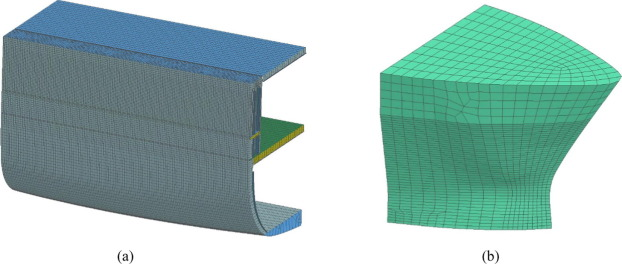
\includegraphics[scale = 1.2]{fig1.jpg}
    \label{fig1}
    \caption{Involved ships for collision analysis: (a) struck ship, and (b) striking ship.\\}
\end{figure*}

These researches are classified in large-analyses as ships are used as observation object. Smaller involved objects was reviewed in crash simulation by finite element analysis \cite{abdel2013frontal} 
and oblique impact scenario of thin-walled tube \cite{manikandaraja2016numerical}. 
In collision study, damage is evaluated which directly receives influence from applied material on its structure or construction. Formulation of material characteristic was addressed in term of hardening parameter \cite{krieg1976implementation}
as in isotropic hardening, the center of the yield surface is fixed but the radius is a function of the plastic strain, strain rate of steel influences yield stress of mild steel which is well known very sensitive to the strain rate 
\cite{jones1993criteria}, and failure, for example as introduced by Jones and Wierzbicki, there are three failure modes that can be experienced by material in experiencing certain load \cite{jones2011structural}. 
These concepts were implemented in present work to observe behaviour of the target object when encountered impact load in form of side collision with other ship. 

\end{document}